\section*{Medici\'on de Campo El\'ectrico {RCEM}}
\paragraph{Preparaci\'on del Equipo - Antenas}
\begin{itemize}
	\item \textbf{Antenas:}
	\begin{itemize}
		\item Toagle Antenna: \'area efectiva $A_e = \frac{\lambda^2 G}{4 \pi}$
		\begin{center}
			\includegraphics[width=0.15\textwidth]{Figures/Toaglas.jpeg}
		\end{center}
		\item ANT 500 Antenna:
		\begin{center}
			\rotatebox{90}{\includegraphics[width=0.06\textwidth]{Figures/ANT500_Antenna.jpeg}}  % Imagen rotada 90 grados
		\end{center}
	\end{itemize}
\end{itemize}

\paragraph{Preparaci\'on del Equipo - Transmisor, Receptor y Software}
\begin{itemize}
	\item \textbf{Transmisor:} USRP B200 mini.
	\begin{center}
		\includegraphics[width=0.15\textwidth]{Figures/B200mini-Large_2.jpg}
	\end{center}
	
	\item \textbf{Receptor:} HackRF One.
	\begin{center}
		\includegraphics[width=0.15\textwidth]{Figures/h1-preliminary1-445.jpeg}
	\end{center}
	
	\item \textbf{Software:} Python para control de transmisi\'on/recepci\'on.
\end{itemize}


%%%%%%%%%%%%%%%%%%%%%%%%%%%%%%%%%%%%%%%%%
\paragraph{Configuraci\'on del Sistema}

\begin{enumerate}
	\item Conectar las antenas al HackRF One.
	\item Configurar el USRP B200 mini con Python para transmitir en las siguientes bandas:
	\begin{itemize}
		\item Servicios Fijos y M\'oviles
		\item FM (88-108 MHz)
		\item TDT (470-790 MHz)
		\item Banda L (1-2 GHz)
		\item 5G (hasta 3.5 GHz)
	\end{itemize}
	\item Configurar HackRF One para recibir en las frecuencias correspondientes.
\end{enumerate}


\centering
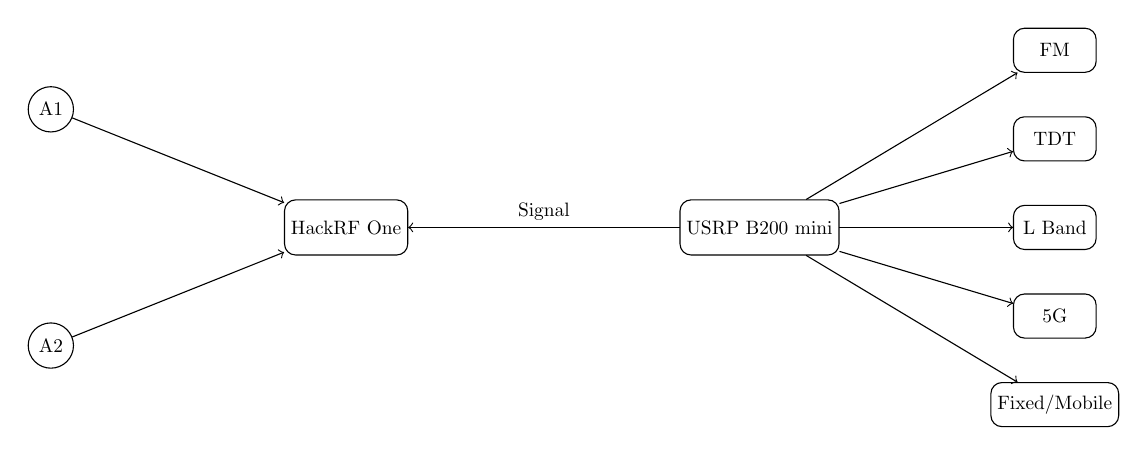
\begin{tikzpicture}[scale=1.5, every node/.style={scale=0.7}]
	% HackRF One
	\node[draw, rectangle, rounded corners, minimum width=2cm, minimum height=1cm] (hackrf) at (0,0) {HackRF One};
	
	% Antennas connected to HackRF One
	\node[draw, circle, minimum size=0.8cm] (antenna1) at (-2.5,1) {A1};
	\node[draw, circle, minimum size=0.8cm] (antenna2) at (-2.5,-1) {A2};
	\draw[->] (antenna1) -- (hackrf);
	\draw[->] (antenna2) -- (hackrf);
	
	% USRP B200 mini
	\node[draw, rectangle, rounded corners, minimum width=2cm, minimum height=1cm] (usrp) at (3.5,0) {USRP B200 mini};
	\draw[<-] (hackrf) -- (usrp) node[midway, above] {Signal};
	
	% Bands
	\node[draw, rectangle, rounded corners, minimum width=1.5cm, minimum height=0.8cm] (band1) at (6,1.5) {FM};
	\node[draw, rectangle, rounded corners, minimum width=1.5cm, minimum height=0.8cm] (band2) at (6,0.75) {TDT};
	\node[draw, rectangle, rounded corners, minimum width=1.5cm, minimum height=0.8cm] (band3) at (6,0) {L Band};
	\node[draw, rectangle, rounded corners, minimum width=1.5cm, minimum height=0.8cm] (band4) at (6,-0.75) {5G};
	\node[draw, rectangle, rounded corners, minimum width=1.5cm, minimum height=0.8cm] (band5) at (6,-1.5) {Fixed/Mobile};
	
	% Connecting bands to USRP
	\draw[->] (usrp) -- (band1);
	\draw[->] (usrp) -- (band2);
	\draw[->] (usrp) -- (band3);
	\draw[->] (usrp) -- (band4);
	\draw[->] (usrp) -- (band5);
\end{tikzpicture}


%%%%%%%%%%%%%%%%%%%%%%%%%%%%%%%%%%%%%%%%%
\paragraph{Procedimiento de Medici\'on}


\begin{itemize}
	\item \textbf{Calibraci\'on inicial:} Medici\'on de se\'nal de referencia.
	\item Captura de datos con HackRF One en cada banda.
	\item Registro de intensidad de campo el\'ectrico con dispositivo manual.
	\item C\'alculo de potencia en dBm con la ecuaci\'on:
	\[
	P_{dBm} = 10 \log_{10}\left( \frac{P_{mW}}{1mW} \right)
	\]
	\item $\eta = 377$ ohmios (impedancia del espacio libre).
\end{itemize}

\begin{table}[ht]
	\centering
	\footnotesize
	\begin{tabular}{cccccc}
		\toprule
		Index & Emisora & Frecuencia (MHz) & Potencia (dBm) & Campo Electrico 377$\omega$ (V/m) \\
		\midrule
		0 & Ol\'impica Stereo & 89.7  & -9.52  & 0.2052  \\
		1 & Radio Nacional de Colombia & 90.1  & -14.29 & 0.1185  \\
		2 & Radio Uno & 91.7  & -8.21  & 0.2386  \\
		3 & La W Radio & 92.5  & -17.09 & 0.0858  \\
		4 & La FM & 94.3  & -5.90  & 0.3114  \\
		5 & Tropicana & 95.5  & -11.61 & 0.1612  \\
		6 & RCN Radio & 98.7  & -15.02 & 0.1089  \\
		7 & La Mega & 100.7  & -14.27 & 0.1188  \\
		8 & Los 40 & 101.7  & -    18.29 & 0.0748  \\
		9 & Radio Tiempo & 102.7 & -15.58 & 0.1022  \\
		\bottomrule
	\end{tabular}
	
	\caption{Datos de las emisoras con sus frecuencias, potencias en dBm y campos electricos a 377$\omega$.}
\end{table}
\clearpage\newpage
%%%%%%%%%%%%%%%%%%%%%%%%%%%%%%%%%%%%%%%%%
\paragraph{Validaci\'on Experimental}


\begin{itemize}
	\item Uso de analizador de espectro y dispositivo de medici\'on de campo manual.
	
	\includegraphics[width=0.3\textwidth]{Figures/ads.jpg}
	
	\item Comparaci\'on de datos entre HackRF One y dispositivos externos.
	
	\begin{minipage}{0.45\textwidth}
		\includegraphics[width=\textwidth]{Figures/104.7_105.7.jpg}
		\includegraphics[width=\textwidth]{Figures/104.7_105.7.png}
	\end{minipage}
	
	\item Calibraci\'on adicional si se encuentra discrepancia.
	\item Confirmaci\'on de precisi\'on en bandas objetivo.
\end{itemize}


%%%%%%%%%%%%%%%%%%%%%%%%%%%%%%%%%%%%%%%%%

\clearpage\newpage
\paragraph{Pruebas en Bandas Espec\'ificas}
\begin{itemize}
	\item \textbf{Servicios Fijos y M\'oviles:}
	\begin{itemize}
		\item C\'alculo de la distancia m\'inima usando la f\'ormula de Fresnel.
		\[
		d = \sqrt{\frac{4 \lambda D}{\pi}}
		\]
		donde $\lambda$ es la longitud de onda y $D$ es la distancia entre las antenas.
	\end{itemize}
	\item \textbf{FM (88-108 MHz):}
	\begin{itemize}
		\item Medici\'on en entorno libre de interferencias.
	\end{itemize}
	\item \textbf{TDT (470-790 MHz):}
	\begin{itemize}
		\item Medici\'on con filtros pasa banda.
	\end{itemize}
\end{itemize}



\vspace{0.5cm}  % Espacio vertical para separar el título del contenido
\small  % Para reducir el tamaño del texto si es necesario
\begin{itemize}
	\item \textbf{Banda L (1-2 GHz):}
	\begin{itemize}
		\item Uso del modelo de Hata para estimar p\'erdidas.
		\[
		PL(dB) = 69.55 + 26.16\log_{10}(f) - 13.82\log_{10}(h_{\text{trans}}) - a(h_{\text{rec}}) + [44.9 - 6.55\log_{10}(h_{\text{trans}})]\log_{10}(d)
		\]
		donde $f$ es la frecuencia en MHz, $h_{\text{trans}}$ y $h_{\text{rec}}$ son las alturas de las antenas, y $d$ es la distancia en km.
	\end{itemize}
	\item \textbf{5G (hasta 3.5 GHz):}
	\begin{itemize}
		\item C\'alculo de la primera zona de Fresnel.
		\[
		r_1 = 17.32 \sqrt{\frac{d}{4f}}
		\]
		donde $r_1$ es el radio de la zona de Fresnel en metros, $d$ es la distancia en kil\'ometros, y $f$ es la frecuencia en GHz.
	\end{itemize}
\end{itemize}
\normalsize  % Para volver al tamaño normal del texto si es necesario


%%%%%%%%%%%%%%%%%%%%%%%%%%%%%%%%%%%%%%%%%
\paragraph{Conclusiones}

\begin{itemize}
	%\item El HackRF One es adecuado para mediciones de RF en varias bandas.
	%\item La calibración adecuada asegura mediciones precisas.
	\item Los resultados son consistentes con dispositivos de medici\'on est\'andar.
	\item Este enfoque es aplicable para an\'alisis en FM, TDT, Banda L y 5G.
\end{itemize}
